\documentclass[10pt,pdftex]{report}
\usepackage[T1]{fontenc}
\usepackage[utf8]{inputenc}
\usepackage[magyar]{babel}
\usepackage{graphicx}
\usepackage{amsmath}
\usepackage{amssymb}
\usepackage{multirow}
\usepackage{booktabs}
\usepackage{indentfirst}
\usepackage[a4paper]{geometry}
\usepackage{url}
\usepackage{titling}
\usepackage{float}
\usepackage{spverbatim}
\usepackage{xcolor}
\usepackage{hyperref}
\usepackage{adjustbox}
    \definecolor{titlebg}{RGB}{128,128,128}

\usepackage{lmodern}
\usepackage{etoolbox}
\patchcmd{\thebibliography}{\chapter*}{\section*}{}{}

\renewcommand{\thesection}{\arabic{section}}


\title{Lineáris erőtörvény vizsgálata}

%% EZ ALÁBBI KÉT MEZŐT ÉRTELEMSZERŰEN KI KELL TÖLTENI
\author{Bíró Gergő Tamás}
\date{2025. április 15.}


%% FEJLÉC LEÍRÓ, NEM KELL MÓDOSÍTANI
\renewcommand*{\maketitle}{\noindent{%
\parbox{\dimexpr\linewidth-2\fboxsep}{\color{black}%
\parbox{\linewidth}{\fontsize{18}{24}\selectfont\sffamily\bfseries\thetitle}%
}}\vskip 1em%
\begin{tabular}{l}%
Mérést végezte: \theauthor \\%
Mérés dátuma: \thedate\\
Jegyzőkönyv végleges változata: \today \\%
Jegyzőkönyv leadásának időpontja: 2025. április 29.
\end{tabular}%
}
%%%%%%%%%%%%%%%%%%%%%

\begin{document}
\maketitle
\section*{Mérés célja}
A mérés során az lineáris erőtörvényt:$F=-Dx$ akarjuk igazolni, ahol $F$ a rugó által kifejtett erő, $D$ a rugóállandó, $x$ pedig a rugó megnyúlása. Ezen kívül a rugók direkciós állandóját is meg akarjuk határozni. Ezeket két különböző módon is lehetséges: a rugók megnyúlásának vizsgálatával, különböző rájuk akasztott súlyok mellett, valamint a rugó rezgésének különböző súlyok melletti periódusidejének vizsgálatával. A mennyiben a feltételezett összefüggés tényleg teljesül meghatározzuk a rugóállandókat mindkét módon, a különböző módszerekkel kapott direkciós állandókat végül összehasonlítjuk.
\section*{Mérőeszközök}
\begin{itemize}
    \item{Állvány}
    \item{Rugók}
    \item{Mérőszalag}
    \item{Egymásra akasztható 50g tömegű súlyok}
    \item{Stopperóra}
\end{itemize}
\section*{A mérés leírása}
Először az első rugót az állványra akasztjuk, ennek megmérjük a kezdeti hosszát, ezután egy 50g tömegű súlyt akasztunk a rugó végére, ekkor is megmérjük a rugó hosszát, és a rugó végén lógó tömeget 50g-al megnöveljük, ezt addig ismételjük, amíg a rugón lévő tömeg nem éri el a 300g-ot. Ezután kicseréljük a rugókat, és a másik rugóval is elvégezzük az előzőeket. Miután a rugók megnyúlásának mérésével végeztünk az egyik rugóra 50g tömegű súly akasztunk, majd azt kicsit kitérítve a rezgés 10 periódusának idejét megmérjük háromszor, majd növeljük 50g-al a tömeget, majd az előzőleg leírt mérést szintén a 300g-os tömeggel bezárólag ismételjük, majd a másik rugóval is elvégezzük.
\section*{Mérési adatok}
\subsection*{1. rugó}
$x_0$\footnotemark$=0.4450m$
\footnotetext{A fellógatott nyújtatlan rugó legalsó pontja mellett a mérőszalagról leolvasható hossz.}
\begin{table}[H]
    \centering
    \begin{tabular}{|r|r|r|}
        \hline
        $m$\footnotemark\footnotetext{A rugóra akasztott súlyok tömege.}$(kg)$ & $x$\footnotemark\footnotetext{A fellógatott rugó legalsó pontja mellett a mérőszalagról leolvasható hossz.}$(m)$ & $\Delta x$\footnotemark\footnotetext{A rugó megnyúlása.}$=x_0-x(m)$ \\
        \hline
        0.05 & 0.4275 & 0.0175 \\
        \hline
        0.10 & 0.4105 & 0.0345 \\
        \hline
        0.15 & 0.3930 & 0.0520 \\
        \hline
        0.20 & 0.3755 & 0.0695 \\
        \hline
        0.25 & 0.3585 & 0.0865 \\
        \hline
        0.30 & 0.3410 & 0.1040 \\
        \hline
    \end{tabular}
    \caption{Az 1. rugó megnyúlása a különböző tomegek mellett.}
\end{table}
\begin{table}[H]
    \centering
    \begin{tabular}{|r|r|r|r|r|r|}
        \hline
        $m(kg)$ & 10 $T_1(s)$ & 10 $T_2(s)$ & 10 $T_3(s)$ & 10 $T_{átlag}(s)$ & $T_{átlag}$\footnotemark\footnotetext{A rugóra rezgésének periódusideje.}$(s)$ \\
        \hline
        0.05 & 3.77 & 3.61 & 3.59 & 3.657 & 0.3657 \\
        \hline
        0.10 & 4.16 & 3.75 & 3.88 & 3.930 & 0.3930 \\
        \hline
        0.15 & 4.56 & 4.60 & 4.59 & 4.583 & 0.4583 \\
        \hline
        0.20 & 5.32 & 5.31 & 5.31 & 5.313 & 0.5313 \\
        \hline
        0.25 & 5.84 & 5.79 & 5.92 & 5.850 & 0.5850 \\
        \hline
        0.30 & 6.39 & 6.47 & 6.25 & 6.370 & 0.6370 \\
        \hline
    \end{tabular}
    \caption{Az 1. rugó rezgésének periódusidejei.}
\end{table}
\subsection*{2. rugó}
$x_0=0.4540m$
\begin{table}[H]
    \centering
    \begin{tabular}{|r|r|r|}
        \hline
        $m(kg)$ & $x(m)$ & $\Delta x=x_0-x(m)$ \\
        \hline
        0.05 & 0.3985 & 0.0555 \\
        \hline
        0.10 & 0.3445 & 0.1095 \\
        \hline
        0.15 & 0.2895 & 0.1645 \\
        \hline
        0.20 & 0.2370 & 0.2170 \\
        0.25 & 0.1830 & 0.2710 \\
        \hline
        0.30 & 0.1295 & 0.3245 \\
        \hline
    \end{tabular}
    \caption{A 2. rugó megnyúlása a különböző tomegek mellett.}
\end{table}
\begin{table}[H]
    \centering
    \begin{tabular}{|r|r|r|r|r|r|}
        \hline
        $m(kg)$ & 10 $T_1(s)$ & 10 $T_2(s)$ & 10 $T_3(s)$ & 10 $T_{átlag}(s)$ & $T_{átlag}(s)$ \\
        \hline
        0.05 & 4.82 & 4.80 & 4.78 & 4.800 & 0.4800 \\
        \hline
        0.10 & 6.72 & 6.74 & 6.87 & 6.777 & 0.6777 \\
        \hline
        0.15 & 8.17 & 8.32 & 8.24 & 8.243 & 0.8243 \\
        \hline
        0.20 & 9.38 & 9.43 & 9.49 & 9.433 & 0.9433 \\
        \hline
        0.25 & 10.49 & 10.55 & 10.45 & 10.497 & 1.04967 \\
        \hline
        0.30 & 11.38 & 11.31 & 11.3 & 11.330 & 1.1330 \\
        \hline
    \end{tabular}
    \caption{A 2. rugó rezgésének periódusidejei.}
\end{table}
A nehézségi gyorsulást $g=9.81\frac{m}{s^2}$ értékűnek tekintjük.
\section*{Hibaforrások}
\begin{enumerate}
    \item{A mérőszalag pontosságából származó hiba.}
    \item{A távolság leolvasásának hibája a rugó kis mértékű rezgése miatt.}
    \item{A stopperóra pontatlansága.}
    \item{Az emberi reakcióidő, amely nagyjából 0.2s, emellett szinte teljesen elhanyagolható az óra hibája.}
    \item{A ridegebb anyagú rugó esetében kis tömegek mellett nehéz pontos időt mérni, így ebben az esetben nagyobb lesz az idő hibája.}
\end{enumerate}
\section*{A mérés kiértékelése}
\subsection*{Rugók megnyúlásának vizsgálata}
Miután a rugókra a súlyt ráakasztottuk, és a rugó egyensúlyban van a súlyra ható erők eredője 0 lesz, tehát a következő egyenlet teljesül: $mg=Dx$, ahol $m$ a súlyok tömege, $D$ a rugóállandó, $x$ a rugó megnyúlása, $g$ pedig a nehézségi gyorsulás. Legyen $y=mg$, ekkor $y=Dx+c$ egyenletű egyenest illesztve az adatainkra azt várjuk, hogy az egyenest jól illeszkedjen a pontokra valamint, hogy $c$ értéke jó közelítéssel 0 legyen, amennyiben ez teljesül a kapott egyenes meredeksége meg fog egyezni a rugóállandóval. Az illesztést elvégezve látható, hogy az egyenesek jól illeszkednek a mért adatokra.
\begin{figure}[H]
    \centering
    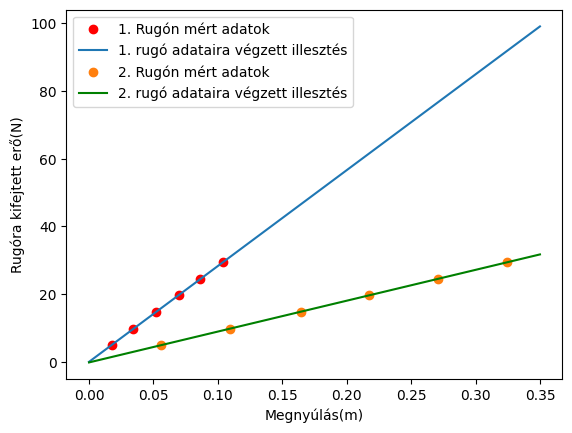
\includegraphics{./megnyulas.png}
    \caption{A megnyúlás vizsgálata során mért adatpontok, és az azokra illesztett egyeneksek.}
\end{figure}
Az első rugó esetében a kapott egyenes paraméterei: $D_1=28.33\frac{N}{m}$, $c_1=-1.85\cdot10^{-3}N$, a másodiknál pedig $D_2=9.21\frac{N}{m}$ és $c_2=-1.94\cdot10^{-2}N$. Mivel mindkét esetben $c$ közel 0 ezért a lineáris erőtörvényt igaznak tekinthetjük. A direkciós állandók hibáját a téglalap módszerrel határozzuk meg:\\
Legyen $y_{ill}$ az illesztés során kapott egyenes által felvett érték adott megnyúlás mellett.
\begin{table}[H]
    \centering
    \begin{tabular}{|r|r|r|r|}
        \hline
        $x(m)$ & $y(N)$ & $y_{ill}(N)$ & $\Delta y=y-y_{ill}(N)$ \\
        \hline
        0.0175 & 0.4905 & 0.4939 & -0.00340 \\
        \hline
        0.0345 & 0.9810 & 0.9755 & 0.00552 \\
        \hline
        0.0520 & 1.4715 & 1.4712 & 0.00026 \\
        \hline
        0.0695 & 1.9620 & 1.9670 & -0.00499 \\
        \hline
        0.0865 & 2.4525 & 2.4486 & 0.00393 \\
        \hline
        0.1040 & 2.9430 & 2.9443 & -0.00132 \\
        \hline
    \end{tabular}
    \caption{$y$, $y_{ill}$ és $\Delta y$ értékei az 1. rugó megnyúlásai mellett.}
\end{table}
\begin{equation*}
    \Delta D_1=2\frac{\left|\Delta y\right|_{max}}{x_{max}-x_{min}}=2\frac{0.00552}{0.1040-0.0175}=0.128\frac{N}{m}
\end{equation*}
Ebből $D_1=28.33\pm0.128\frac{N}{m}$. A második rugó esetében ugyaníg határozhatjuk meg a hibát:
\begin{table}[H]
    \centering
    \begin{tabular}{|r|r|r|r|}
        \hline
        $x(m)$ & $y(N)$ & $y_{ill}(N)$ & $\Delta y=y-y_{ill}(N)$ \\
        \hline
        0.0555 & 0.4905 & 0.4868 & 0.00366 \\
        \hline
        0.1095 & 0.9810 & 0.9794 & 0.00159 \\
        \hline
        0.1645 & 1.4715 & 1.4811 & -0.00961 \\
        \hline
        0.2170 & 1.9620 & 1.9510 & 0.00200 \\
        \hline
        0.2710 & 2.4525 & 2.4526 & 0.00007 \\
        \hline
        0.3245 & 2.9430 & 2.9406 & 0.00242 \\
        \hline
    \end{tabular}
    \caption{$y$, $y_{ill}$ és $\Delta y$ értékei a 2. rugó megnyúlásai mellett.}
\end{table}
\begin{equation*}
    \Delta D_2=2\frac{\left|\Delta y\right|_{max}}{x_{max}-x_{min}}=2\frac{0.00961}{0.3245-0.0555}=0.071\frac{N}{m}
\end{equation*}
Így $D_2=9.21\pm 0.071 \frac{N}{m}$ adódik.
\subsection*{Rugók rezgésének vizsgálata}
Kis kitérések mellett rezgő rugó periódusidejét a következő képlet adja meg:$T=2\pi\sqrt{\frac{\mu}{D}}$, amely lineáris erlőtörvényt felhasználva vezethető le. Ebben $T$ a rezgés periódusideje, $D$ a rugóállandó és $\mu=m+m_{eff}$ ahol $m$ a rugóra akasztott súlyok tömege $m_{eff}\sim \frac{m_r}{3}$ pedig a rugó effektív tömege, ahol $m_r$ a rugó tömege. Ezt átrendezve a következő egyenletre juthatunk:
\begin{equation*}
    m=\frac{DT^2}{4\pi^2}-m_{eff}
\end{equation*}
Legyen $u=m$, $v=\frac{T^2}{4\pi^2}$ és $m_{eff}=w$, ekkor $u$-ra $v$ függvényében egyenest illesztve annak meredeksége meg fog egyezni $D$-vel, amennyiben illeszkedik az adatokból kiszámolt pontokra.
\begin{table}[H]
    \centering
    \begin{tabular}{|r|r|}
        \hline
        $u(kg)$ & $v(s^2)$ \\
        \hline
        0.05 & 0.00339 \\
        \hline
        0.10 & 0.00391 \\
        \hline
        0.15 & 0.00532 \\
        \hline
        0.20 & 0.00715 \\
        \hline
        0.25 & 0.00867 \\
        \hline
        0.30 & 0.01029 \\
        \hline
    \end{tabular}
    \caption{$u$ és $v$ értékei az 1. rugó esetében.}
\end{table}
\begin{table}[H]
    \centering
    \begin{tabular}{|r|r|}
        \hline
        $u(kg)$ & $v(s^2)$ \\
        \hline
        0.05 & 0.00584 \\
        \hline
        0.10 & 0.01163 \\
        \hline
        0.15 & 0.01721 \\
        \hline
        0.20 & 0.02254 \\
        \hline
        0.25 & 0.02799 \\
        \hline
        0.30 & 0.03252 \\
        \hline
    \end{tabular}
    \caption{$u$ és $v$ értékei a 2. rugó esetében.}
\end{table}
Az 1. rugó anyaga nagyon rideg, ezért az arra kapott $v$ értékek $u=0.05kg$ és $u=0.10kg$mellett pontatlalnok, így a rugóállandó pontosabb meghatározásához azokat az illesztés során figyelmen kívül hagyjuk.\\
Az 1. rugó adataira végzett illesztés paraméterei a következők: $D_1=30.43\frac{N}{m}$, és $w_1=-0.0143kg$, amennyiben az első két pontot is figyelembe vennénk $D_1=34.01\frac{N}{m}$ adódik, amely jóval nagyobb a nyúlás során kapott meredekségnél, így tényleg jogos azokat a pontokat elhagyni. A második rugónál $D_2=9.31\frac{N}{m}$ és $w_2=-0.00773kg$ paramétereket kapunk. Az illesztések jól láthatóan illeszkednek az adatpontjainkra, így ezzel a módszerrel is sikerült igazolni a lineáris erőtörvényt.
\begin{figure}[H]
    \centering
    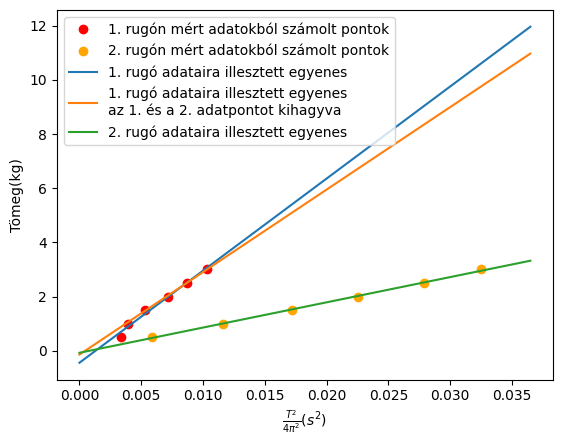
\includegraphics{./rezges.png}
    \caption{A mérések során kapott értékekből számított $u$ és $v$ értékek, valamint az azokra illesztett egyenesek.}
\end{figure}
A durkciós állandók hibáját ismét a téglalap módszerrel határozzuk meg, legyen $u_{ill}$az illesztésből kapott egyenes által felvett érték az egyes $v$-kben és $\Delta u = u-u_{ill}$.
\begin{table}[H]
    \centering
    \begin{tabular}{|r|r|r|r|}
        \hline
        $v(s^2)$ &  $u(kg)$ & $u_{ill}(kg)$ & $\Delta u(kg)$ \\
        \hline
        0.00532 & 0.15 & 0.148 & 0.0022 \\
        \hline
        0.00715 & 0.20 & 0.204 & -0.0036 \\
        \hline
        0.00867 & 0.25 & 0.250 & 0.0002 \\
        \hline
        0.01028 & 0.30 & 0.299 & 0.0012 \\
        \hline
    \end{tabular}
    \caption{$u$, $u_{ill}$ és $\Delta u$ értékei $v$ függvényében az 1. rugónál.}
\end{table}
Ebből:
\begin{equation*}
    \Delta D_1=2\frac{\left|\Delta u\right|_{max}}{v_{max}-v_{min}}=2\frac{0.0036}{0.01028-0.00532}=1.45\frac{N}{m}.
\end{equation*}
Tehát $D_1= 30.43\pm1.48\frac{N}{m}$.
\begin{table}[H]
    \centering
    \begin{tabular}{|r|r|r|r|}
        \hline
        $v(s^2)$ &  $u(kg)$ & $u_{ill}(kg)$ & $\Delta u(kg)$ \\
        \hline
        0.00584 & 0.05 & 0.047 & 0.0033 \\
        \hline
        0.01163 & 0.10 & 0.101 & -0.0007 \\
        \hline
        0.01721 & 0.15 & 0.153 & -0.0027 \\
        \hline
        0.02254 & 0.20 & 0.202 & -0.0023 \\
        \hline
        0.02791 & 0.25 & 0.252 & -0.0024 \\
        \hline
        0.03252 & 0.30 & 0.295 & 0.0047 \\
        \hline
    \end{tabular}
    \caption{$u$, $u_{ill}$ és $\Delta u$ értékei $v$ függvényében a 2. rugónál.}
\end{table}
\begin{equation*}
    \Delta D_2=2\frac{\left|\Delta u\right|_{max}}{v_{max}-v_{min}}=2\frac{0.0047}{0.03252-0.00584}=0.35\frac{N}{m}.
\end{equation*}
Amiből $D_2=9.31\pm0.35\frac{N}{m}$
\subsection*{eredmények}
\begin{table}[H]
    \centering
    \begin{tabular}{|r|r|r|}
        \hline
        Megatározás módja & $D_1\left(\frac{N}{m}\right)$ & $D_2\left(\frac{N}{m}\right)$ \\
        \hline
        Rugó nyújtása & $28.33\pm0.128$ & $9.21\pm 0.071$ \\
        \hline
        Rugó rezgetése & $30.43\pm1.48$ & $9.31\pm0.35$ \\
        \hline
    \end{tabular}
    \caption{A rugóállandókra kapott értékek.}
\end{table}
\section*{Diszkusszió}
A mérés során sikeresen igazoltuk a lineáris erőtörvényt mindkét módszerrel. A 2. rugó esetében egymáshoz nagyon közeli rugóllandókat kaptunk a két módszer segítségével, azonban az 1. rugóra nagyobb az eltérés, amelyet feltehetően az okozott, hogy annak anyaga nagyon rideg, így nehéz volt pontosan megmérni a rezgésének periódusidejét, ebből a mérési hibából származó hiba okozta a jelentős eltérést a végeredményel különbségében.

\end{document}
%rúd téglalap